\documentclass[final,3p,sort&compress,12pt]{elsarticle}

%% The amssymb package provides various useful mathematical symbols
\usepackage{amssymb}
\usepackage{setspace}
\usepackage{pifont}
\usepackage{amsmath}
\usepackage{amsfonts}
\usepackage{pgf-pie}
\usepackage{pgfplots}
\usepackage{calc}
\usepackage{graphicx}
\usepackage{float}
\usepackage{anyfontsize}
\usepackage{pgfplots}
\usepackage{comment}
\usepackage{booktabs}
\usepackage{rotating}
\usepackage{siunitx}
\usepackage{eurosym}
\usepackage{multirow}
\usepackage{xcolor} 
\usepackage{colortbl}
\usepackage{subcaption}
\usepackage{blindtext}


\bibliographystyle{elsarticle-num-names} 

\DeclareSIUnit{\EUR}{\text{\euro}}
 \pgfplotsset{compat=1.17}


\journal{Energy and Buildings}

\begin{document}

\begin{frontmatter}

%% Title, authors and addresses

\title{Developing decarbonisation pathways for Irish homes in changing TIMES}


\author[inst1,inst2]{Jason Mc Guire \corref{j.mcguire@ucc.ie}}
\cortext[j.mcguire@ucc.ie]{j.mcguire@ucc.ie}

\affiliation[inst1]{organization={Energy Policy and Modelling Group, MaREI Centre},
            addressline={Environmental Research Institute}, 
            city={Cork},
            country={Ireland}}
            
\affiliation[inst2]{organization={School of Engineering},
            addressline={University College Cork}, 
            city={Cork},
            country={Ireland}}

\author[inst1,inst2]{Fionn Rogan}
\author[inst1,inst2]{Olexandr Balyk}
\author[inst1,inst2]{Tomás Mac Uidhir}
\author[inst1,inst2]{Ankita Gaur}
\author[inst1,inst2]{Brian Ó Gallachóir}
\author[inst1,inst2]{\& Hannah Daly}

 \onehalfspacing
\begin{abstract}
%% Text of abstract

Ireland has committed to one of the most ambitious decarbonisation targets in the world to 2030. The residential sector, responsible for 14.2\% of total greenhouse gas (GHG) emissions \cite{Howley2020Energy-RelatedIreland.} , is among the most carbon intensive per dwelling in the EU, emitting 60\% more $CO_2$ than the national EU average \cite{SustainableEnergyAuthorityofIreland2018EnergySector}, because of a high share of low thermal efficient detached dwellings coupled with a high dependency on carbon-intensive heating fuels. These factors have served as barriers to the decarbonisation of the residential sector in Ireland to date.  The TIMES-Ireland Model (TIM) is a newly developed optimisation model for the Irish energy system. This paper describes the innovative methodology applied to the development of the residential sector in TIM and explores the results, which provides new insights on optimal residential decarbonisation pathways.

\vspace{0.25cm}
\noindent

\end{abstract}

\begin{keyword}

Energy Systems Optimisation Model \sep TIMES \sep Residential decarbonisation \sep Model description 

\end{keyword}

\end{frontmatter}

%% \linenumbers
\newpage
%% main text
 \onehalfspacing
\section{Introduction}
\label{sec:Introduction}

The Introduction section of this paper reviews Energy System Optimisation Models (ESOMs) which use a bottom-up or hybrid approach and include all energy-related sectors, and bottom-up residential sector models which have have a detailed level of technological representation. The hybrid approach combines bottom-up technological detail and top-down macroeconomic detail. The introduction also analyses Ireland's distinctive residential sector, climate targets, and current energy policy. 

 \onehalfspacing
\subsection{Energy Systems Optimisation Modelling and the Residential Sector}
\label{Intro:ESOM}

Economically optimal or least cost residential decarbonisation pathways are dynamic, advancements in heating technologies, new low-carbon fuel alternatives and new heating technologies continuously alter the optimal pathway. ESOMs have a rich representation of existing and future technological variables such as efficiency, cost, and fuel, while also accounting for macroeconomic variables such as economic growth and the social discount rate. ESOMs supply enough energy to at least satisfy each energy service, while also considering sectoral interconnections to explore optimal decarbonisation pathways. There are a number of widely used ESOMs, such as MESSAGE \cite{Messner1995Model-basedPlanning}, TIMES \cite{Loulou2016DocumentationI}, Balmorel \cite{Wiese2018BalmorelModel}, TEMOA \cite{Hunter2013ModelingTemoa} and OSeMOSYS \cite{Howells2011OSeMOSYS:Development.}. 

These models can be used to explore the residential sector in high spatial, temporal and technological granularity. Different levels of disaggregation are applied to the residential sector in models, \citet{Natarajana2011ModellingApproach}  highlighted a common approach used by defining an average performance for a number of dwelling categories. To account for the heterogeneous mix of dwellings, each dwelling is categorised based on building type to better reflect the housing stock and provide building specific insights. Some models also disaggregate the year of construction \cite{Ahern2013StateStock}, wall type \cite{Dineen2015ImprovedSource} and level of insulation \cite{Clinch2001Cost-benefitEfficiency}.

% Average dwellings -	Would it be worth having a paragraph early in this section that describes some relevant characteristics of the residential sector, e.g. very heterogeneous mix of dwelling types (hence the archetype approach), a slow turnover of building stock (hence challenge of very ambitious near term targets), a broad distinction between new and existing dwellings (former very efficient, latter often not efficient), different types of energy use (space heating, water heating, appliances), drivers of energy demand (weather, affluence, demographics), non-economic rationality of dwelling occupants (hence caution required with techno-economic modelling approaches)? This might help frame your review. - Fionn


The Integrated MARKAL-EFOM System (TIMES) has been extensively used in both the UK and Ireland, and there are several examples of using TIMES to focus on the residential sector. TIMES assumes perfect foresight to enable a least-cost solution to be calculated, but \textit{``in reality, the behaviours of consumers is not always economically rational"} \cite{Li2018IncorporatingModel}. In light of this,  \citet{Li2018IncorporatingModel} investigated the heating technology preference in the UK using UK TIMES Model (UKTM) by incorporating a Discrete Choice Model (DCM) to better reflect how homeowners choose heating technologies and thus addressing for simplification of the perfect foresight assumption.

There is a rising tendency for ESOMs to focus on new building fabric \cite{Leibowicz2018OptimalServices,Dineen2011ModellingHeating} and retrofitting to thermally improve the existing residential stock \cite{Dineen2015ImprovedSource}. Another trend observed is the electrification of energy-related sectors \cite{Chiodi2013ModellingSystem}, while a focus on photovoltaic (PV) systems can be examined in parallel \cite{Marczinkowski2018ResidentialSystems}. The strength of an ESOM can be used to examine the sectoral interactions, one study by Hedegard and Münster \cite{Hedegaard2013InfluenceOperation} examined the interaction between heat pumps and wind generation investments in Denmark, the results find it is optimal to install air-to-water heat pumps in non-DH areas. 


\subsubsection{Ireland: Residential Modelling}
\label{Intro:ESOMIreland}

ESOMs have been used to optimise Ireland's entire energy system \cite{Chiodi2013ModellingSystem,Connolly2009DevelopingUniversity.}, however no Irish studies use ESOMs to solely explore the residential sector, as many models look across multiple sectors. However, two examples of Irish ESOMs focusing the residential sector in higher granularity are outlined below.

In 2014, \citet{Rogan2014LEAPsSystem} linked OSeMOYOS to the Long Range Energy Alternatives Planning system (LEAP), which is a scenario-based simulation modeling tool used to analysis energy policy in all sectors of the economy. The models were linked to explore specific energy efficiency policies in the residential and other sectors. Three scenarios were explored, namely, the reference scenario, energy efficiency scenario, and energy efficiency+ scenario, while three residential policies were analysed retrofitting, building regulation and lighting. At the time of this study little to no data on retrofits existed and the Building Energy Rating (BER) public database was much smaller. \citet{Rogan2014LEAPsSystem} research focuses on the theoretical energy savings from retrofits, \textit{with both the
number of dwellings and the scale of improvement
works specified exogenously from the model} \cite{Rogan2014LEAPsSystem}, the model limited retrofits to BER bands D to G while not accounting for internal temperature shifts.
The reference scenario assumes that 300,000 existing dwellings will undergo a shallow retrofit from 2009 to 2020, and the results show that residential total energy consumption rose 6.7\% in 2020, compared to 2008. In the energy efficiency scenario, 800,000 residential dwellings are retrofitted, resulting in a 9.9\% reduction of energy consumption compared to the reference scenario. The energy efficiency+ scenario allows for the same quantity of retrofits, but accounts for deeper retrofits resulting in an energy consumption reduction of 16.5\%, compared to the reference scenario. The insights highlight the importance of the depth of retrofit, as shown by the results. The model also found considerable scope for energy savings to be made through improved building regulations. 

In 2018, \citet{Thellufsen2019ImplementingIreland} investigated the potential for the implementation of District Heating (DH) in both the commercial and residential sectors of Ireland. The paper analyses the $CO_2-80$ scenario ( 80\% $CO_2$ reduction in 2050, compared to 1990 ) with and without DH using the previous Irish TIMES model and EnergyPLAN. The previous version of Irish TIMES did not account for DH, so EnergyPLAN is used to investigate the operation and  feasibility of DH in Ireland. A sensitivity analysis was performed on investment costs, heat grid losses, and discount rates. In all cases, the inclusion of DH was found to be favourable. The results find the conversion of 37\% of the Irish heat demand to DH to be optimal. Both the TIMES model and climate target used in this study are superseded and the study did not include the future heat savings expected from retrofitting, nevertheless this study has provided insights on the potential of DH.

\par  The majority of previous modelling on the residential sector in Ireland has involved bottom-up residential sector models, which are not optimisation models. These models have provided insights on the input data, methodology, and results. In the first comprehensive analysis of the Irish residential sector, Clinch and Healy examined fuel poverty \cite{Healy2002FuelIreland}, excess winter mortality \cite{Clinch2000HousingMortality}, market failures \cite{Clinch2000DomesticFailure}, occupancy behaviour \cite{Clinch2001ModellingEfficiency}, social benefit \& cost \cite{Clinch2001Cost-benefitEfficiency}  and energy efficiency  \cite{Clinch2003ValuingModel,Clinch2001Cost-benefitEfficiency,Clinch2001ModellingEfficiency}. 

\par
In 2011,  \citet{Dineen2011ModellingHeating} developed a residential bottom-up model to assess the impacts of measures in Ireland's National Energy Efficiency Action Plan (NEEAP). The model focused on new buildings and examined the energy efficiency of space and water heating by examining technology and building fabric thermal efficiency.  %The paper acknowledges that retrofitting of existing stock will play a large role in meeting energy efficiency targets, however it is not examined, nor is the internal temperature effect on energy efficiency improvements. 
Later in 2015, \citet{Dineen2015ImprovedSource} built on previous work in examining new dwellings, by examining the energy savings potential of energy efficiency improvement measures in the existing dwelling stock. The Dwelling Energy Assessment Procedure (DEAP) model was used, this is the national tool for the BER calculation. A complete set of filters was applied to the BER database before use in the model, erroneous and outlining data was removed. \citet{Dineen2015ImprovedSource} performed and sensitivity analysis and found that there was a 7.5\% change in energy consumption for every 1$^{\circ}$C internal temperature shift. Concluding, BER standard assumptions are poor as they vastly overestimate dwelling energy consumption, the average internal temperature across the Irish dwelling stock may be closer to 18$^{\circ}$C than 21$^{\circ}$C.
\par In 2013, \citet{Ahern2013StateStock} investigated thermal retrofit measures of the existing detached, oil centrally heated, rural housing stock. %A base geometry according to age bands and thermal characteristics was created in the study. The default values used in some of the BER database variables where highlighted. For example, there are assumed U-values when the roof insulation thickness is unknown, this is based on age, but there are no U-values for uninsulated roofs despite a 2001 survey finding 18\% of detached housing in Ireland had no roof insulation. 
\citet{Ahern2013StateStock} found dwellings built post-2000 consume the greatest amount of energy (kWh/annum), due to their large floor area. Concluding that the majority of thermal energy efficiency progress in Irish dwellings is being offset. The model results show that thermal improvement measures resulted in a reduction of running costs and $CO_2$ emissions by an average of 65\% for houses constructed prior to 1979, compared to houses built in 1979 or after resulting in an average 26\% reduction in running costs and $CO_2$ emissions from retrofit measures. This study highlights the potential energy savings within pre-1979 oil centrally heated, rural housing stock. 
\par The Archetype Dwelling Energy Model - SQL (ArDEM-SQL) developed by Mac \citet{Uidhir2020ImprovingDecisions} converts the Irish BER public database into Microsoft SQL language to calculate the annual energy consumption for space/ water heating, and lighting using EN 13790:2004 to simulate the potential for improved energy efficiency gains within an existing retrofit program. Mac \citet{Uidhir2020ImprovingDecisions} examined the Better Energy Homes (BEH) retrofit grant scheme. 
%The five most common retrofit combinations were simulated for 9 distinct archetypes (3 BER energy rating groups, and 3 building types) and compared these to alternative retrofit combinations which delivered additional efficiency improvements. 
The results show that the alternative retrofit scenarios can achieve additional energy efficiency gains of up to 86\%, relative to the set of retrofit combinations actually delivered from the program. This shows the the type of retrofit(s) and archetype can have a large affect on the energy saved.   

\par Finally, the Sustainable Energy Authority of Ireland's (SEAI’s) National Energy Modelling Framework (NEMF) is a suite of modelling tools used for modelling the Irish energy system. The SEAI is Ireland's national energy authority and they \textit{provide evidence-based advice across the government, state and semi-state bodies, in addition to delivering a range of grant and support programmes to promote sustainable energy} . The models listed are some of the models used within SEAI's NEMF to model the impact of incentives and opportunities created by specific policy instruments. 


\begin{enumerate}[1.]
\item {Core Structural Model of the Irish Economy (COSMO)  is a macro-economic model used by the Economic and Social Research Institute (ESRI) to create a baseline forecast of energy consumption by sector} \cite{Bergin2017COSMO:Ireland}
\item{PLEXOS is a power systems modeling tool used for electricity modeling and planning} \cite{2021PLEXOSExemplar}
\item{Energy-efficiency policy analysis tool informs the energy efficiency estimates} \cite{Scheer2015UnlockingOpportunity}
\begin{enumerate}[i.]
\item{Complementary to the Energy-efficiency policy analysis tool is the Consumer Choice Model which determines the attractiveness of energy efficiency finance options}\cite{SustainableEnergyAuthorityofIreland2017BehaviouralSector}
\end{enumerate}
\item{BioHEAT is a techno-economic simulation model of bioenergy and heat} \cite{Durusut2018BioHEAT:Sectors}
\end{enumerate}

The models described in this section include a range of national ESOMs and bottom-up residential models with varied objectives. The complexity of models has increased significantly in the last 20 years, in Ireland, the models started out in Microsoft Excel and switched to Microsoft SQL, the higher computational power allows for deeper analyses. The growing BER database is provides detailed open sourced data for input to Irish models. 
%The internal temperature is becoming more frequently analysed in Irish residential studies, a recurring theme is the wide range of internal temperatures which Dineen et al. \cite{Dineen2015ImprovedSource} found this assumption significantly changes the final residential energy consumption.


\subsection{Case study for Ireland}
\label{Intro:IreRSD}

\subsubsection{Residential sector characteristics}
\label{Intro:GHG}

Under 2006 Intergovernmental Panel on Climate Change (IPCC) guidelines, Ireland’s residential sector accounted for 14.2\% of GHGs emissions in 2018 \cite{Howley2020Energy-RelatedIreland.}. Focusing only on energy-related GHG emissions from heat, electricity and transport, the residential sector directly accounts for 24\% of GHG emissions. The residential sector is directly responsible for 47\% of heat and 30\% of electricity and indirectly responsible for a share of the remaining GHGs, especially in the transport sector, as the rural settlement patterns increase transport demands. 

Ireland’s distinctive energy sectors are further separated from other EU member states when focusing on the residential sector. This is largely down to rural settlement patterns, larger dwellings, lower building thermal efficiency, and higher reliance on fossil fuels. This is illustrated by the fact only 5.8\% of the population of Ireland were living in apartments in 2018, the lowest in EU-27 and well below the 25.3\% average \cite{Eurostat2021DistributionSurveyilc_lvho01}, furthermore 71.4\% of the Irish population are deemed to be living in dwellings too large, where the EU-27 rate is 33\% \cite{Eurostat2021ShareSurveyilc_lvho50a}. The low thermal efficiency of Ireland's dwelling stock is highlighted by two facts; (i) 2021 building regulations require a 70\% reduction of $CO_2$ emissions in new dwellings compared to dwellings built in 2005 \cite{DepartmentofHousing2021Gov.ieBuildings}, and (ii) Central Statistics Office (CSO) data states approx. 85\% of residential buildings are 2005 or older. Additionally, Ireland's fossil fuel dependency is underpinned by home heating oil, which accounts for the largest share of fuel usage in the residential sector at 37\% \cite{SustainableEnergyAuthorityofIreland2018EnergySector}, of which all is imported \cite{OCleirigh2020EnergySEAI}.

In the last 30 years, the extraction of indigenous peat has declined and consequently peat consumption has halved, in 2018 peat accounted for 12.3\% of residential GHG emissions. GHG emissions from coal in the residential sector also declined to 6.9\% in 2018 \cite{Howley2020Energy-RelatedIreland.}. However, the decline in peat and coal has been offset by a more significant growth in oil in the same period, where oil accounted for 34.8\% of residential GHG emissions in 2018 \cite{Howley2020Energy-RelatedIreland.}. Despite being limited to some urban areas, gas still accounted for 15.5\% of residential GHG emission in 2018 \cite{Howley2020Energy-RelatedIreland.}. 
The residential sector relied on fossil fuels for over 90\% of thermal energy in 2018, consequently Ireland currently has the lowest renewable heat among EU member states, at only 6.3\% \cite{Eurostat2021ShareSourcesnrg_ind_ren}. %Preliminary results from the Environmental Protection Agency (EPA) have indicated a 9\% increase of residential GHG emissions in 2020, mainly due to low home heating oil prices and covid-related restrictions, proving some consumers are economically rational by filling oil tanks when prices are low. 

Space and water heating are the main energy services, accounting for 80\% of the energy used in residential dwellings \cite{SustainableEnergyAuthorityofIreland2018EnergySector} and typical heating systems have a lifetime of at least 15 years, consequently leading to a slow turnover of technology in the residential sector. Apart from space and water heating, all EU member states are required under commission regulation (EU) 431/2014 to supply energy consumption data on space cooling, cooking, lighting \& appliances, and others (mainly outdoor appliances), the annual trend of these energy services is shown in Fig. \ref{fig:IrelandServiceDemands}.

% Space heating is the largest residential energy service, which accounted for 61.8\% of final energy usage in 2018. Other residential energy services and their share of final energy are shown in Fig.\ref{fig:Ireland2018ServiceDemands}. As building thermal efficiency and heating technology efficiency improves, both space and water heating energy would be expected to decline. 


\begin{figure}[!ht]
\centering
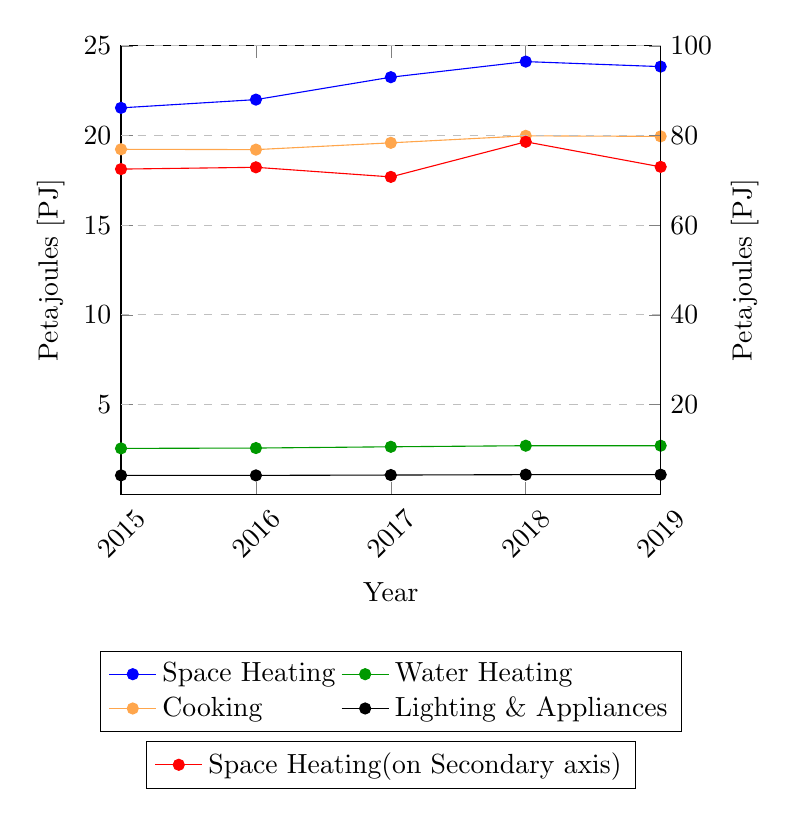
\begin{tikzpicture}
\begin{axis}[
    scale=1,
    legend cell align={left},
    x tick label style={/pgf/number format/1000 sep=,rotate=45},
    legend style={at={(0.5,-0.35)},anchor=north,legend columns=2},
    xlabel={Year},
    ylabel={Petajoules [PJ]},
    xmin=2015, xmax=2019,
    ymin=0, ymax=25,
    xtick={2015,2016,2017,2018,2019},
    ytick={5,10,15,20,25},
    ymajorgrids=true,
    grid style=dashed,
]

\addplot[
    color=blue,mark=oplus*
    ]
    coordinates {
    (2015,21.54)(2016,22)(2017,23.25)(2018,24.12)(2019,23.84)
    };
    
\addplot[
    color=green!60!black,mark=oplus*
    ]
    coordinates {
    (2015,2.55)(2016,2.57)(2017,2.64)(2018,2.7)(2019,2.7)
    };
\addplot[
    color=blue!60,orange!70, mark=oplus*
    ]
    coordinates {
    (2015,19.23)(2016,19.211)(2017,19.59)(2018,19.98)(2019,19.95)
    };
\addplot[
    color=black,mark=oplus*
    ]
    coordinates {
    (2015,1.046)(2016,1.045)(2017,1.065)(2018,1.086)(2019,1.084)
    };
    \legend{Space Heating,Water Heating,Cooking,Lighting \& Appliances, Other}
    
\end{axis}
%
\begin{axis}[
scale=1,
    scale=1,
    legend cell align={left},
    x tick label style={/pgf/number format/1000 sep=,rotate=45},
    legend style={at={(0.5,-0.55)},anchor=north,legend columns=2},
    xmin=2015, xmax=2019,
    ymin=0, ymax=100,
    xtick={2015,2016,2017,2018,2019},
    ytick={20,40,60,80,100},
    ymajorgrids=true,
    grid style=dashed,
    axis y line*=right,
    axis x line=none,
    ylabel style = {align=center},
    ylabel= {Petajoules [PJ]}
]

\addplot[
    color=red,mark=oplus*
    ]
    coordinates {
    (2015,72.5)(2016,72.9)(2017,70.76)(2018,78.59)(2019,73)
    };
    
     \legend{Space Heating(on Secondary axis)}
    \end{axis}
\end{tikzpicture}
\caption{Ireland Residential Energy Service Demands \cite{Eurostat2021Disaggregatednrg_d_hhq}}
\label{fig:IrelandServiceDemands}
  \end{figure}  






\subsubsection{Policy context}
\label{Intro:Policy}

Under the Climate Action and Low Carbon Development (Amendment) Act 2021, the Irish government has adopted legally binding national targets to reduce GHG emissions by 51\% in 2030, compared to 2018. The Act also proposes a long-term target to achieve a climate neutral economy or ``net-zero" by 2050 \cite{2021Climate2021}. These targets account for all emissions - both Emission Trading System (ETS) emissions and non-ETS emissions, and sets out to make sectoral five-year carbon budgets a legal requirement to aid progress of the forementioned long-term targets. 
\par The EU's first Nationally Determined Contribution (NDC), which had a 40\% GHG reduction target (first NDC), has been succeeded by a new target of at least a 55\% GHG reduction target (updated NDC) by 2030 compared to 1990 levels. Ireland's Climate Action Plan 2019 (CAP2019) complies with the EU's first NDC, from which Irelands 30\% Non-ETS GHG reduction target in 2030 compared to 2005 levels was derived  \cite{DepartmentofCommunicationsClimateActionandEnvironment2019Climate2019}. Climate Action Plan 2021 will be more ambitious than its predecessor, CAP2019 as it must reflect EU's updated NDC target and take account of the national target also.
There are also renewable energy targets to consider for transport (RES-T), heat (RES-H), and electricity (RES-E) under the renewable directive (EU) 2018/2001, and the energy efficiency targets under (EU) 2018/2002.

The Irish government's long-term overarching strategy aims to  achieve \textit{``effective density and consolidation, rather than more sprawl of urban development, [as] a top priority"}\cite{Ireland2018ProjectFramework}. The densification of Ireland's main cities will provide opportunities to improve the efficiency of heating, electricity, and transport within and between cities. The Marginal Abatement Cost Curve (MACC) produced in CAP2019, shows electricity \& transport are the most cost-effective sectors for energy decarbonisation \cite{DepartmentofCommunicationsClimateActionandEnvironment2019DecarbonisationIreland}. In Ireland, the decarbonisation of electricity is underway, with carbon intensity falling annually to 375 $gCO_2/kWh$ in 2018, which is 40\% lower than 2005 levels \cite{Howley2020Energy-RelatedIreland.}. 
Ireland uses both the \textit{carrot} (subsidy) and \textit{stick} (tax) approach to direct private investment towards low carbon or renewable energy. A €15/ $tCO_2$ carbon tax was introduced in 2009 to reduce investment in fossil fuels, and the increasing carbon tax rate has resulted in tax receipts growing every year from 2010 to 2018 \cite{Oireachtas2019AnOffice}. Ireland's current carbon tax of €33.50/ $tCO_2$ is set to rise to €100/ $tCO_2$ in 2030. The Renewable Energy Feed-in Tariff (REFIT) schemes were designed to incentivise renewable electricity investment to achieve legally binding renewable targets under 2009/28/EC. The Renewable Electricity Support Scheme (RESS) replaced REFIT in 2020. RESS supports renewable electricity projects to help Ireland achieve 2030 climate targets, especially the 70\% renewable electricity target. 

\par As the grant provider, SEAI plays a key role in the rollout of retrofitting and heat pumps. The retrofitting and heat pump grants do still require large upfront costs from the consumer, which may hinder the ambitious targets as this wont be a viable option for many households, green loans are currently available to bridge this gap and other options are being explored. % are therefore the preferred heating technology despite the high capital costs. CAP2019 planned to retrofit 500,000 existing homes to at least a  ‘B2’ energy rating by 2030, which highlights the energy efficiency first approach in the residential sector. 
Gas Network Ireland (GNI) have set a 18\% biomethane target for 2030 \cite{Ervia2019VisionIreland}, where CAP2019 only set a 3\% biomethane target for 2030 \cite{DepartmentofCommunicationsClimateActionandEnvironment2019Climate2019}. %GNI anticipates that by 2026 or 2027 the supply from Corrib ( Irelands only indigenous gas supply, which provided 61\% of gas in 2018 ) will be less than 30\% of 2018 levels \cite{OCleirigh2020EnergySEAI}. 
A major barrier to increasing biomethane from an agricultural source in the gas network is the cost, it was the most expensive option in the MACC produced in CAP2019.
Ireland has one of the lowest shares of DH in Europe at less than 1\%  \cite{Gartland2016AIreland}. %
%Advancement in DH control and awareness of the technology will strengthen the case for DH networks to play a part in decarbonising the residential sector.
CAP2019 plans to have 0.4\% of heating provided by DH in 2030. The Irish District Energy Association (IrDEA) suggest 57\% of heat can be sourced from DH, if supporting policy and regulation was in place. CAP2019 sets out a need to develop a policy framework for the development of DH in Ireland.
%DH will likely play a role, however, Gartland points out a range of organisational, technical, regulatory, and economic barriers to DH growth in Ireland \cite{Gartland2016AIreland}. 

\subsection{Motivation \& Paper Overview}
\label{Intro:PaperOver}

The distinctive Irish residential sector provides an interesting case study and new Irish climate targets now means previous Irish models which relied on superseded climate targets are out-dated, but not redundant. A new iteratively built transparent ESOM with wide stakeholder involvement, which aligns with current climate policy is needed to robustly explore optimal decarbonisation pathways and technical limits. 
The new model will provide opportunity for deeper analysis of the energy system sectors, with accessible soft-linking capabilities. The model development process can be applied to any national or regional ESOM.  
No such ESOM with a focus on Irish residential sector exists, the strength of an ESOM is to account for sectoral interactions which bottom-up simulation models cannot provide. Structural improvements and archetypes in the model aligns with existing retrofitting and electrification strategies. Other model innovations include filtering the BER database, other EU countries with publicly available BER database under directive (EU) 2018/844 can apply similar methods, while TIM also considers internal temperatures shifts and new energy service demands were calculated. TIM can provide a robust methodology into \textit{``how Ireland should set GHG targets in the residential sector”} and TIM will be a critical tool in exploring \textit{how changes to future technology developments affect the optimal residential heating decarbonisation pathway in Ireland? }.

The layout of the rest of this paper is as follows; section \ref{Meth} is the core section of this paper and explains the methodology used to develop the residential sector. The treatment of input data in the model is described, the calculations are explained, and assumptions and constraints are highlighted. Section \ref{Results} outlines the scenarios used and displays results from the residential sector. Section \ref{Discussion} discusses the results, strengths, and weakness of the newly developed model and how it differs from other models. Section \ref{Conclusion} draws some conclusions and discusses possible future work.

%brings together sections 1.1 and 1.2 – one paragraph justifying this study (improving residential modelling; applying to important case study), and include the objectives of the study (introduce the model and any research questions) then bring the paragraph on the structure from the start. This is a bridging section between the introduction and methodology. - Hannah 

\section{Methodology}
\label{Meth}



\subsection{TIMES}
\label{MethTIMES}

\par  The expertise among energy policy researchers in Ireland combined with the global network of Energy Technology Systems Analysis Program (ETSAP) modellers, makes TIMES the preferred ESOM to explore Ireland's decarbonisation pathways. Previous versions of the Irish TIMES model were extracted from the Pan European TIMES model and then updated with specific national data and assumptions, to provide informative reports on Irish climate policy \cite{Gallachoir2012EPAModel,Deane2017Irish2,Gallachoir2020The3,Deane2013TechnicalIreland,IrishGovernment2017National2017}. The previous Irish TIMES model was non-transparent and inflexible model, which was not purpose built for the Irish energy system. The introduction of new climate policies and targets combined with technological advancements pushed the need for a new model, however the need for a transparent, flexible and robust model, purpose built for the Irish energy system by Irish energy modellers was a key driver to develop a new model.The new ``TIMES Ireland Model" (TIM) was built in 2021 to address this need \textbf{(SOURCE)}.
\par TIMES is a bottom-up optimisation energy-environment model with perfect foresight which is used to analyse various levels of spatial, temporal and sectoral resolution. Exogenous technical, physical, and regulatory constraints can be applied and technologies have specified fuel types, efficiency, lifetime, availability, environmental characteristics, and fixed, variable and operation costs. TIMES uses a linear programming optimizer matrix in General Algebraic Modeling System (GAMS), to compute all calculations. 

\par The function of partial equilibrium operates whereby the prices and quantities in each time period are such that the suppliers produce exactly the quantities demanded by the consumers and therefore the total economic surplus  (sum of the suppliers’ and consumers’ surpluses) is maximized \cite{Loulou2016DocumentationI}. The TIMES objective is therefore to minimize the total cost of the system, by solving for the following:
\begin{equation} 
\begin{split}
NPV = {\sum_{r=1}^{R}  \sum_{y\in YEARS}(1 + d_{r,y})^{REFYR-y}}
\cdot {ANNCOST(r,y)} 
\end{split}
%\[ \sum_{n=1}^{\infty} 2^{-n} = 1 \]
\label{Eq:ObjectiveFunction}
\end{equation}

Where, $NPV$ is the net present value of the total cost for all regions ; $ANNCOST(r,y)$ is the total annual cost in region r and year y; $d_{r,y}$ is the general discount rate; $REFYR$ is the reference year for discounting; YEARS is the set of years for which there are costs; and $R$ is the set of regions in the area of study.

\subsection{TIMES-Ireland Model (TIM)}
\label{Meth:TIM}


TIM was developed completely online during national lockdowns, with no face to face meetings, the model relied on git-centred model development process with different developers leading different sectors. Weekly meetings were combined with intensive daily ``sprint" meetings to keep model milestones on track. The transparency of TIM improved the iterative development process, external energy experts and other stakeholders contributed using web-based dashboards\footnote{https://tim-review1.netlify.app/results/}. The schematic in Fig. \ref{fig:TIMOverviewRES} shows the main sectors of the model, represented in the demand-side modules and how they link with the supply-side modules, to create a full picture of the national energy system \textbf{SOURCE}.

\begin{figure}[!htbp]
 \centering
 \includegraphics[width=\textwidth]{Figures/TIMOverviewRES.jpg}
 \caption{Structure of TIM }
 \label{fig:TIMOverviewRES}
\end{figure}

TIM is set up with regional options, either one national region or 26 county regions, and with different temporal resolution options, only the national annual results were explored in this study.

\subsection{TIM: Residential Sector}
\label{Meth:TIMRes}


The residential sector was developed with awareness of the ongoing national retrofitting and electrification strategies and investments. The residential energy services were developed based upon regulation (EU) 431/2014, shown in Fig. \ref{fig:IrelandServiceDemands}, however there is no space cooling data available in Ireland and lighting \& appliances are separated in TIM, while ``others" was combined with appliances. An overview of the flow of energy from fuels to demand, through the energy services is shown in Fig. \ref{fig:RES}.  

\begin{figure}[!htbp]
 \centering
 \includegraphics[width=\textwidth]{Figures/TIM_RES3.png}
 \caption{Structure of TIM residential sector }
 \label{fig:RES}
\end{figure}

The BER database provides the base year bottom-up energy consumption data, this is scaled up to represent the entire stock and cross-checked with the top-down energy consumption from the 2018 SEAI Energy Balance. To compare the two databases, fuels were were merged and separated, with 13 fuels adequately covering the residential sector in TIM, Table \ref{AppTable:Fuels} summarizes the fuels from the different data sources. In TIM, fuels such as ``coal", represent a combination of fuels from the SEAI Energy Balance and BER database. Gasoil which has similar properties to kerosene, is accounted for in the SEAI Energy Balance,  but there is no evidence to support keeping gasoil and kerosene separate would provide further insight into residential decarbonisation, therefore these fuels are combined in TIM. However, disaggregating ambient heat could potentially provide insights on residential decarbonisation, so the model has separated space ambient heat and water ambient heat. The solid multi-fuel from the BER database represents an open fire or stove which is heated by either coal, peat, or wood. Through examining the SEAI Energy Balance and BER database, the fuel share for coal, peat, and wood in solid multi-fuel was set to 19.4\%, 74.4\% and 6.2\% respectively. 
\par There are two types of energy services represented in Fig. \ref{fig:RES} - Non-Archetype and Archetype. Essentially Non-archetype energy services have a lack of data and could not be accurately assigned to an archetype. The six non-archetype energy services are not dependant on the type of dwelling in the model and the base year quantity is the total national consumption of that energy service. Non-Archetype data was retrieved from SEAI Residential Energy Report \cite{SustainableEnergyAuthorityofIreland2018EnergySector} and cross-checked with the POTEnCIA database and the top-down data from the SEAI Energy Balance, more details on non-archetype services are found in Section \ref{Meth:Data}. The four archetype energy services and the internal temperature adjustment are dependent on  building type and data is sourced from the BER database, which is discussed in Section \ref{Meth:Data}. The demand for archetype and non-archetype energy services is based on the growth of residential dwellings, which is also detailed in Section \ref{Meth:Data}. 

\subsubsection{Data}
\label{Meth:Data}
%
The dwelling stock data is obtained from the SEAI BER Public database\footnote{https://ndber.seai.ie/BERResearchTool/ber/search.aspx}, is filtered then scaled up using Central Statistics Office (CSO) data. 
The SEAI BER public database is Ireland's national Energy Performance Certificate (EPC) register,  which complies with the Energy Performance of Buildings Directive 2018/844/EU (EPBD). The BERs are categorised based on expected energy consumption, with A1 representing the lowest expected energy consumption ($\leq 74 kWh/m^2/year$) and G representing the highest expected energy consumption ($ >450 kWh/m^2/year$). Over half of all Irish dwellings are captured in the BER database and every BER displays over 200 energy related variables. The DEAP model which is used to assign BER labels,  is outlined by \citet{Dineen2015ImprovedSource} in Section \ref{Intro:ESOM}. In terms of space heating, DEAP assumes that each dwelling is single zoned, the heating times are 7am to 9am and 5pm to 11pm ( 56 hours / week ) during the heating season, which is from October to May inclusive and assumes monthly external temperatures, the average external temperature assumed for the heating season is 7.6$^{\circ}$C. However, one assumption, the internal temperature assumption, results in a large unsupportable error, where space heating is overestimated by 26\%, this is a simliar finding to \citet{Dineen2015ImprovedSource} who found a 7.5\% change in energy consumption for every 1$^{\circ}$C shift in internal temperatures. After internal temperature adjustments in Table \ref{Table:InternalTemps} were applied in TIM, this brought the final energy consumption in line with the top-down SEAI Energy Balance. DEAP assumes that living areas ( living room, sitting room, and possibly kitchen) in all dwellings are heated to 21$^{\circ}$C and non-living areas ( bedroom, bathroom, hallways ) are heated to 18$^{\circ}$C. Through the analysis of previous residential modelling in Ireland internal temperatures are often much lower than 21$^{\circ}$C in living areas and 18$^{\circ}$C in non-living areas \cite{Dineen2015ImprovedSource,Healy2002FuelIreland,Clinch2003ValuingModel,Clinch2000HousingMortality}.

\begin{table}[htbp]
  \centering
  \footnotesize
  \caption{Internal Temperature Assumptions}
    \begin{tabular}{rrr}
    \hline
    \multicolumn{1}{l}{BER Rating} & \multicolumn{1}{l}{Living Area} & \multicolumn{1}{l}{Non-Living Area }  \\ \hline
    A  & 23$^{\circ}$C   & 20$^{\circ}$C  \\
    B  & 21$^{\circ}$C   & 18$^{\circ}$C  \\
    C  & 18$^{\circ}$C  & 15$^{\circ}$C  \\
    D  & 18$^{\circ}$C   & 15$^{\circ}$C  \\
    E  & 18$^{\circ}$C   & 15$^{\circ}$C  \\ 
    F  & 18$^{\circ}$C   & 15$^{\circ}$C  \\ 
    G  & 18$^{\circ}$C   & 13$^{\circ}$C  \\ \hline
    \end{tabular}
  \label{Table:InternalTemps}
\end{table}

The ArDEM-SQL, which was described in section \ref{Intro:ESOMIreland} is a simulation model built on space heating calculation EN 13790. ArDEM-SQL alters the primary energy consumption of the BER database by changing the internal temperatures assumed by DEAP in Table \ref{Table:InternalTemps}. Other concerns for uncertainties in the database, which are not related to DEAP calculation are statistically anomalous spikes in the data, caused by applying default values \cite{Ahern2020ADatabases} and different companies generating variations of ±20\% in the assessment of energy consumption \cite{Harsman2016OnCertificates}. While the BER database provides high granularity data, it must be filtered to improve the representation of the dwelling stock data. The filters applied to the raw BER database are outlined in Table \ref{AppBERFilters}. 
%PICKUPHERE
The Census 2016 data \cite{CentralStatisticsOffice2016CensusIreland} from the CSO is also used in calculating the dwelling stock, dataset E1005 provides a split of seven building archetypes per county, which are aggregated to form three building archetypes in TIM. The total number of dwellings per archetype per county in 2016 is used to scale up the BER database. The gap in total dwellings between the census year in 2016 and the model base year in 2018 was initially ignored due to lack of data. However, later it was found that data on new dwelling electrical connections per archetype and per county are available from CSO dataset NDQ06, this would have filled the gap, the first iteration of the dwelling stock in TIM does not account for the 2\% of existing dwellings build in 2017 and 2018. 
\par Once the BER database and CSO database tables have been filled to include dwellings per archetype per county, the next step was to scale up the BER database. This was done by first finding the ratio of the building archetype per county between the BER database and CSO data, as shown in Equation \ref{Eq:BERtoCSO1}.

\begin{equation} 
\begin{split}
R_{a,c} = {\frac{CSO_{a-nsa,c}} {BER_{a,c}} + \frac{CSO_{nsa,c}} {CSO_{a,c}}}
\end{split}
\label{Eq:BERtoCSO1}
\end{equation}

$R_{a,c}$ is the ratio per archetype (a) and per county (c), there are 26 counties and 3 archetypes. $CSO_{a-nsa,c}$ represents the number of dwelling archetypes minus the non-stated archetypes (nsa) per county in the CSO database. $BER_{a,c}$ is the number of archetypes per county  in the BER database. The next step is to multiply the number of BERs per archetype and per county by the relevant ratio.
\begin{equation} 
\begin{split}
TIM_{a,c} = BER_{a,c} * R_{a,c} 
\end{split}
\label{Eq:BERtoCSO2}
\end{equation}

$TIM_{a,c}$ represents the final dwelling stock data per archetype and per county, the first iteration of TIM does not disaggregate the dwellings per county, instead a national total per archetype is input to TIM ( $TIM_a$ ).


Once the final dwelling stock is complete, the next step is to assign a BER rating to all dwellings. This was done by comparing nine different dwelling age ranges for each of the three archetypes between the BER and CSO datasets. 


\begin{equation} 
\begin{split}
TIM_{r,y,a} = CSO_{y,a} * \frac{BER_{r,y,a}} {BER_{y,a}} * \frac{TIM_{a}} {BER_{a}}
\end{split}
\label{Eq:AgeBER}
\end{equation}

Where $TIM_{r,y,a}$ is the total dwellings in TIM by BER rating (r), year of construction (y), and archetype (a). $CSO_{y,a}$ is the number of dwellings by year of construction and archetype in the CSO dataset, no BER rating types exist in the CSO dataset. $BER_{r,y,a}$ is the number of BER ratings by year of construction and archetype from the BER database and dividing this value by $BER_{y,a}$ results in a probability of a certain age type falling within a BER rating, and the final part of the equation $\frac{TIM_{a}} {BER_{a}}$ compensates for the non-stated archetypes in the CSO data, $TIM_a$ was already calculated in Equation \ref{Eq:BERtoCSO2}. The results of each of the BER probablities are summarized for each archetype in  Table \ref{AppBERCor},\ref{AttBERCor} \& \ref{DetBERCor}, while Table \ref{Table:FinalDwellingStock} outlines the final dwelling stock used in TIM. 


\begin{table}[htbp]
  \centering
  \footnotesize
  \caption{TIM Base Year Dwelling Stock}
\begin{tabular}{l|lll}
BER Rating & Apartment & Attached & Detached \\ \hline
A          & 9,419     & 15,472   & 20,379   \\
B1         & 7,459     & 9,538    & 9,434    \\
B2         & 14,042    & 17,545   & 20,091   \\
B3         & 19,924    & 49,769   & 53,466   \\
C          & 58,905    & 282,152  & 251,319  \\
D          & 43,739    & 187,627  & 166,668  \\
E          & 25,768    & 101,419  & 81,397   \\
F          & 12,331    & 50,124   & 43,241   \\
G          & 15,211    & 52,707   & 78,436   \\ \hline
Total      & 206,799   & 766,352  & 724,430 
\end{tabular}
\label{Table:FinalDwellingStock}
\end{table}


The costs applied in the residential sector, includes space and water heating technologies, retrofitting, cooking, lighting, pumps, fans, space cooling, and other electrical appliances. 
The majority of the space and water heating cost data is obtained from the
\textit{``Techno-economic projections until 2050 for smaller heating and cooling technologies in the residential and tertiary sectors in the EU”} report \cite{JointResearchCentre2017Techno-economicEU}, the report has spatial cost data and the north EU region (Denmark) was mainly used \cite{JointResearchCentre2017Techno-economicEU}, this cost data is sourced from the continuously updated and expanding Danish Energy Agency's Technology Data for Individual Heat Production dataset and where data was missing, the central EU region (Germany) cost data was used \cite{JointResearchCentre2017Techno-economicEU}. The high granularity of data allows for the cost of a technology to be disaggregated between apartments and non-apartments, costs and efficiencies are projected every five years from 2020 to 2050. The lifetime and emissions/pollutants are also included, while the cost data is further disaggregated between capital expenditure ( equipment, installation \& additional capital costs ) and Operational \& Maintenance (O\&M) costs. 
The cost data for different electrical appliances is sourced from Topten EU database \cite{Michel2016EnergyREPORT} and SEAI \cite{SustainableEnergyAuthorityofIreland2018EnergySector}. Topten has a large database covering electrical appliances available in the European market, the data collected includes cost and efficiency of refrigeration, cloth washing, cloth drying, and dish washing, while some Topten reports have looked at sales and European market shares \cite{Michel2016EnergyREPORT}. Cooking data is sourced from Eurostat's ``Energy consumption in households by type and end-used"  \cite{Eurostat2021Disaggregatednrg_d_hhq} and cross-checked with SEAI \cite{SustainableEnergyAuthorityofIreland2018EnergySector}. Appliances not included in this list are simply under the ``Electrical Appliances" category in TIM. Electrical Appliances include television, multimedia, outdoor appliances, and computer technology and data is sourced from SEAI \cite{SustainableEnergyAuthorityofIreland2018EnergySector} and Eurostat \cite{Eurostat2021Disaggregatednrg_d_hhq}. The fuel costs are not applied in the residential sector, there are applied in the supply sector, and the data is sourced from World Energy Outlook reports from 2019 \cite{/content/publication/caf32f3b-en} and 2020 \cite{/content/publication/557a761b-en}.  
\par TIM has two types of retrofitting options per archetype,  a shallow retrofit is when the primary energy ($kWh/m^2/yr$) is reduced by $ \leq 35\%$, and deep retrofit is where the primary energy is reduced by $>35\%$, while a reduction of $ \ >75\%$ is considered infeasible. The difference between the pre-retrofit and post-retrofit primary energy determines the type of retrofit, as shown in Table \ref{AppDepthofRetrofit}. The retrofit cost data was sourced from Ali et. al \cite{Ali2020ABuildings} who derived costs from SEAI's Better Energy Homes (BEH) and Better Energy Warmer Homes (BEWH) datasets, combined this is Ireland's largest retrofitting dataset ( over 285,000 retrofits ). To provide more robust retrofit costs, data is also used from the Typology Approach for Building Stock Energy Assessment (TABULA) report \cite{IrishTABULANationalAdvisoryGroup2014BuildingIreland} which has more detailed cost data with two stages of retrofit (standard and advanced) for a sample of 31 dwellings. The formulas used to find the average cost of a retrofit per type of retrofit and archetype are shown in Equations \ref{Eq:RetrofitCost1} and \ref{Eq:RetrofitCost2}.

\begin{equation} 
\begin{split}
 \text{\euro}_{rf-rt,a} = Average ( (Ali_{rf-rt} * AF),TABULA_{rf-rt,a} )
\end{split}
\label{Eq:RetrofitCost1}
\end{equation}

Where $ {\text{\euro}}{}_{rf-rt,a}$ is the retrofit cost from pre-retrofit BER rating or rating from (rf) to post-retrofit rating or rating to (rt) for archetype (a). $Ali_{r,t}$ is the cost data from  \citet{Ali2020ABuildings}, it contains all BER ratings and retrofit types but does not include an archetype, so an archetype factor (AF) is introduced, 0.9 for apartments, 1 for attached, and 1.1 for detached dwellings.  $TABULA_{rf-rt,a}$ is the average retrofit cost from pre-retrofit BER rating to post-retrofit BER rating for an archetype, data is sourced from TABULA \cite{IrishTABULANationalAdvisoryGroup2014BuildingIreland}.  However with only 62 samples in total not all retrofits are included. In this case, TABULA is ignored and \citet{Ali2020ABuildings} is the only source of retrofit costs. The retrofit costs are cross-checked with the residential cost-optimal report \cite{AECOM2020ReportBuildings}. 
\par To simplify the model, the cost of retrofit per BER rating is not used in TIM. Instead, an average weighted cost per archetype and per retrofit is calculated. 

\begin{equation} 
\begin{split}
\text{\euro}_{a,t} = Average(\text{\euro}_{rf,a}) * \frac{TIM_{r,a}} {TIM_{a}}
\end{split}
\label{Eq:RetrofitCost2}
\end{equation}

${TIM_{r,a}}$ is the number of dwellings by rating and archetype and ${TIM_{a}}$ is the total number of dwellings of that archetype, however A-rated dwellings are excluded from the total, as it is assumed they cannot be retrofitted further. So $ {\text{\euro}}{}_{a,t}$ is the average weighted cost per type of retrofit per archetype, which is used in TIM. 


The previous paragraphs outlined the cost of retrofitting and the expected savings of retrofitting in existing dwellings is now examined, along with building regulations savings in new dwellings.  
The annual heating costs per archetype and per BER rating are sourced from SEAI's indicative energy running costs. The internal temperature assumptions in Table \ref{Table:InternalTemps} are included to calculate the costs, which are outlined in Table \ref{Table:FuelCost}

\begin{table}[htbp]
  \centering
  \footnotesize
  \caption{Annual heating fuel cost per BER rating and archetype }
    \begin{tabular}{l|lcc}
    \hline
    BER Rating & Attached & \multicolumn{1}{l}{Detached} & \multicolumn{1}{l}{Apartment} \\ \hline
A1         & $\text{\euro}$323      & $\text{\euro}$539                          & $\text{\euro}$200               \\
A2         & $\text{\euro}$646      & $\text{\euro}$1078                         &$\text{\euro}$400                \\
A3         & $\text{\euro}$804      & $\text{\euro}$1213                         & $\text{\euro}$500                 \\
B1         & $\text{\euro}$745      & $\text{\euro}$1200                         & $\text{\euro}$440              \\
B2         & $\text{\euro}$950      & $\text{\euro}$1500                         & $\text{\euro}$570                \\
B3         & $\text{\euro}$1150     & $\text{\euro}$1900                         & $\text{\euro}$700                \\
C1         & $\text{\euro}$862      & $\text{\euro}$1432                         & $\text{\euro}$499              \\
C2         & $\text{\euro}$1022     & $\text{\euro}$1693                         & $\text{\euro}$624           \\
C3         & $\text{\euro}$1181     & $\text{\euro}$1888                         & $\text{\euro}$686                \\
D1         & $\text{\euro}$1434     & $\text{\euro}$2364                         & $\text{\euro}$836                \\
D2         & $\text{\euro}$1701     & $\text{\euro}$2769                         & $\text{\euro}$964               \\
E1         & $\text{\euro}$1979     & $\text{\euro}$3233                         & $\text{\euro}$1187               \\
E2         & $\text{\euro}$2252     & $\text{\euro}$3646                         & $\text{\euro}$1319                \\
F          & $\text{\euro}$2740     & $\text{\euro}$4403                         & $\text{\euro}$1626              \\
G          & $\text{\euro}$2702     & $\text{\euro}$4398                         & $\text{\euro}$1687        \\                  \hline
    \end{tabular}
  \label{Table:FuelCost}
\end{table}


As TIM only inputs the savings per type of retrofit and archetype, some calculations must be performed on Table \ref{Table:FuelCost} to estimate the savings from retrofits. The first calculation is to find the savings from pre-retrofit running cost to post-retrofit running cost, as shown in Equation \ref{Eq:RetrofitSaving1}

\begin{equation} 
\begin{split}
 Saving(\%)_{a,rf-rt} = 1 - ( \frac {Average(\text{\euro}_{rt,a}/year) } {Average(\text{\euro}_{rf,a}/year) } )
\end{split}
\label{Eq:RetrofitSaving1}
\end{equation}

Where $Saving(\%)_{a,rf-rt}$ are the savings ( or reduced running cost) per archetype (a), where the pre-retrofit BER rating is defined as the rating from (rf), and the post-retrofit BER rating is defined as the rating to (rt). Allocating each retrofit change to either shallow or deep is the next step, this is shown in Table \ref{AppDepthofRetrofit}. The next calculation is to find the weighted average of each retrofit depth per archetype, this is then a TIM input. 

\begin{equation} 
\begin{split}
Saving(\%)_{a,t} = Average(Saving(\%)_{a,rf}) * \frac{TIM_{r,a}} {TIM_{a}}
\end{split}
\label{Eq:RetrofitSaving2}
\end{equation}

Where t is the type of retrofit. ${TIM_{r,a}}$ is the number of dwellings by rating and archetype and ${TIM_{a}}$ is the total number of dwellings of that archetype. The expected savings from each type of retrofit and for each archetype are outlined in Table \ref{Table:RetrofitSavings}.

\begin{table}[htbp]
  \centering
  \footnotesize
  \caption{Retrofit Savings}
\begin{tabular}{l|lcc}
Retrofit & Attached & \multicolumn{1}{l}{Detached} & \multicolumn{1}{l}{Apartment} \\ \hline
Shallow  & 20\%   & 20\%     & 22\%     \\
Deep     & 44\%   & 42\%     & 37\%               
\end{tabular}
\label{Table:RetrofitSavings}
\end{table}


The  technical  bottom-up  development  approach  of  the  residential  sector  is  combined with other economic sectors to meet macroeconomic defined demands. The energy service demands in the residential sector are driven by the total dwelling stock for non-archetype energy services and apartment, attached or detached for archetype energy services. The residential stock projections up to 2040 are taken from ESRI's housing demand estimates \cite{Bergin2020RegionalLevel}, beyond 2040 the growth rate is extrapolated. However, the archetype specific growth is limited or unavailable, for this reason a simple linear regression, as shown in Eq. \ref{Eq:RegArchetype} is used to calculate the share of an archetype in a given year (y).  This is graphically represented in Fig. \ref{fig:DwellingStoc}. The growth rate of apartments is the highest and increasing up to 2040, while the growth in attached and detached dwellings are lagging behind. The obsolescence rate of the existing dwellings is taken as 0.35\%.

\begin{figure}[!htbp]
 \centering
 \caption{Number of dwellings by type and age ('000)}
 \includegraphics[width=\textwidth]{Figures/TIM_DwellingStock.png}
 \label{fig:DwellingStoc}
\end{figure}

\begin{equation} 
\begin{split}
Apt(\%) =  7.5\ln{(y)} -56.97 \\
Att(\%) = -2.53\ln{(y)} + 19.68 \\
Det(\%) = -4.93\ln{(y)} + 37.91
\end{split}
\label{Eq:RegArchetype}
\end{equation}


Archetype energy service demands are dependant on both the type of dwelling and whether it is existing or new. The average archetype energy service demand in new and existing is shown in Table \ref{Archetype Energy Service Demands}.

\begin{table}[htbp]
  \centering
  \footnotesize
  \caption[width=\textwidth]{Archetype Energy Service Demands}
 \begin{tabular}{c|cc|cc|cc}
 \hline
 \multicolumn{1}{c|}{Energy Service}  & \multicolumn{2}{c|}{Apartments} & \multicolumn{2}{c|}{Attached} & \multicolumn{2}{c}{Detached}  \\
  \multicolumn{1}{c|}{}  & \multicolumn{2}{c|}{($kWh/house/yr$)} & \multicolumn{2}{c|}{($kWh/house/yr$)} & \multicolumn{2}{c}{($kWh/house/yr$)}  \\
  & Existing & New & Existing & New & Existing & New \\
 \hline
 Space Heating & 3,853 & 1,228 & 7,852 & 2,845 & 14,405 & 6,745 \\
 Water Heating & 3,409 & 2,197 & 3,011 & 2,351 & 3,806 & 2,493 \\
 Lighting & 179 & 156 & 254 & 229 & 419 & 392  \\
 Pumps \& Fans  & 55  & 60 & 106 & 104 & 131 & 110  \\
 Space Cooling  & 0 & 60 & 0 & 104 & 0 & 110  \\
 \hline
 \end{tabular}
 \label{Archetype Energy Service Demands}
\end{table}

The base year heating energy consumption is derived from the BER database, but uses census data \cite{CentralStatisticsOffice2016CensusIreland} from the CSO dataset E1008 to calibrate the fuel used in heating systems per archetype. Space heating, water heating, and lighting energy service demands for existing dwellings are calculated from the average values of the base year dwelling stock, and as all new dwellings are required to be A-rated, the energy service demand for new dwellings in TIM is calculated from the average of the existing A-rated dwellings. The pumps \& fans energy demands are calculated in a similar method, except in the new dwellings the value is halved and the remaining half is added to space cooling, this aligns with POTEnCIA's (Policy Oriented Tool for Energy and Climate Change Impact Assessment) space cooling and pump \& fan projections per household. While the demands are exogenous, the choice of technologies to at least satisfy the demand are endogenous and is captured in Eq. \ref{Eq:Technology}.

\begin{equation} 
\begin{split}
Min \text{\euro} \sum_k VAR\_ACT_{k,i}(y)  \geq DM_i(y) 
\end{split}
\label{Eq:Technology}
\end{equation}

Where VAR\_ACT are the activity levels of end-use technology (k) for demand category (i) in year (y). DM is the exogenous demand per energy service per year. The cost of the technology is minimised while also satisfying all constraints. All space and water heating technologies are archetype specific and some technologies deliver both water and space heating, while other technologies can only deliver one type of heating, the list of available technologies is outlined in Table \ref{AppHeatingTech}. Retrofits are included as they satisfy the residential space heating demand, even though retrofits do not consume fuel similar to a solar water heating system, from that perspective. In Appliances  unlike in the heating energy service demands, there is little or no choice in different technologies (k) for some of the demand categories (i), therefore, the model is restricted in lighting, appliances and pumps \& fans. However, the cost and efficiency of each technology does determine the overall investment. 

``User Constraints" are defined as any combination of constraints including fixed, maximum or minimum bounds on growth, investment or shares on technologies or fuels. The ``User Constraints" applied to better align with the residential sector include:
\begin{enumerate}[1.]
 \item Only one space and water heating system per household ( stoves excluded ), this user constraint is applied to represent individual heating systems and calibrate results.
 \item Maximum 60\% of existing buildings to be retrofitted by 2030, and 95\% by 2070, the maximum value is interpolated between 2030 and 2070. This is user constraint is applied to align with maximum available labour and was applied during the model development to calibrate results. 
 \item A prerequisite requirement for electrical heat pump installation is applied to each archetype. Table \ref{tab:HeatPumpConstraint} shows the percentage of dwellings which requires a shallow or deep retrofit before a heat pump can be installed (  A heat pump ready dwelling must be at least a B2 rating). Hybrid heat pumps are not included in this constraint, as they can supply higher water temperatures without significantly reducing performance. This user constraint was applied because of the lack of data regrading electrical heat pumps in less than B2 rated dwellings, without this constraint heat pumps are installed in poorly rated dwellings, this constraint aligns with known heat pump performance data.   
 \begin{table}[htbp]
  \centering
  \footnotesize
  \caption{Prerequisite Heat Pump Requirement}
    \begin{tabular}{r|rrr}
    \hline
    \multicolumn{1}{l}{Requirement} & \multicolumn{1}{l}{Apartment} & \multicolumn{1}{l}{Attached } & \multicolumn{1}{l}{Detached} \\ \hline
    No Retrofit  & 24.5\%   & 14.3\%   & 12\% \\
    Shallow Retrofit  & 28.5\%   & 34.7\%  & 36.8\% \\
    Deep Retrofit  & 47\%   & 51\%  & 51.2\% \\
    \end{tabular}%
  \label{tab:HeatPumpConstraint}%
\end{table}%
 \item For space and water heating, each archetype has an upper gas growth constraint of 40\% higher than the base year value. This user constraint was applied in advance of the model development to align with gas infrastructure development. 
\item Maximum fuel share in cooking for gas and LPG is 40\% and 10\% respectively. Base year fuel share for Gas is 32\% and LPG is 1.5\%. This user constraint was applied in advance of the model development to align with gas infrastructure development.
\item Maximum 10\% solar input to dual fuel heating technology. This constraint was applied based on technological constraints.
\item Maximum 30\% gas input to gas hybrid heating pumps. This constraint was applied based on technological constraints.
\end{enumerate}

While other constraints are applied in different sectors, which affect the residential sector and vice versa, they are not listed in this paper. The growth constraints listed above are calculated using the following \cite{Loulou2016DocumentationI} : 
\begin{equation} 
\begin{split}
VAR\_CAP(t + 1) \leq (1 + G^{M(t+1)-M(t)}) \cdot VAR\_CAP(t)
\end{split}
\label{Eq:GrowthConstraint}
\end{equation}

Where $VAR\_CAP$ is the technology capacity in time period (t), G is the growth coefficient, defined as a new attribute of the technology and represents the maximum annual growth allowed for the capacity. The quantity $M(t+1)-M(t)$ is the number of years between the milestones of time periods t and t+1. 


\section{Results}
\label{Results}

The results from TIM can provide some valuable insights on the residential sector and the sectoral interconnections in achieving long-term climate targets. While the purpose of this paper was to describe the residential methodology, the results used here only scrape the surface in terms of exploring residential decarbonisation. However, the results provide some initial insights into residential decarbonisation and are discussed in section \ref{Discussion}. Two different scenarios are used to explore the results and those scenarios and descriptions detailed here:

\begin{enumerate}[(a)]
    
    \item \textbf{Previous Effort } complies with Climate Action Plan 2019, reduces Non-ETS GHG by 30\% in 2030 compared to 2005, and post-2030 targets are forward extrapolated.
    \item \textbf{Current Effort} complies with Climate Action Bill 2021, energy system GHG emissions reduces by 65\% by 2030 compared to 2018 \& net-zero in 2050 ( complies if agriculture GHG emissions reduces by 25\% in 2030 ).
\end{enumerate}


\subsection{Residential Results}
\label{Results:Residential }

The quantity and mix of fuel going into the residential for each scenario and year is  shown in Fig. \ref{fig:ResFuel}. The base year is shown on the left, while annual snapshots of the fuel-mix for the other scenarios are shown for 2030, 2040, and 2050. 

In 2018, the residential sector required 124 PJ of primary energy, the increase in households, and energy efficiency improvements resulted in a 9\% primary energy increase in 2030, under the Previous Effort scenario. Whereas under the Current Effort scenario, the primary energy is required to reduce by 13\% in 2030, this highlights the large incremental step in ambition required when moving from Climate Action Plan 2019 to the Climate Action Bill 2021. In 2050, under the Previous Effort scenario, the total primary energy shows a continued growth 17\% higher than 2018, whereas the Current Effort scenario shows an overall reduction of 11\% which indicates a post-2030 growth, highlighting the high ambition in the 2030 target. 

\begin{figure}[!htbp]
 \centering
 \includegraphics[width=\textwidth]{Figures/residential_fuelmix.png}
 \caption{Residential fuel-mix per scenario per year}
 \label{fig:ResFuel}
\end{figure}

The fluctuation in the fuel-mix required is significant, especially to comply with 2030 targets, for example, oil reduces 60\% in the Previous Effort and 90\% in the Current Effort scenario in 2030. Furthermore, peat and coal are phased out completely in the residential sector in both scenarios in 2030. The lesser carbon intensive natural gas increases by 211\% in Previous Effort without the upper constraint of the gas infrastructure and decreases 4\% in Current Effort scenario. The electricity continues to decarbonise rapidly in all scenarios, resulting in an increase in electricity in the residential sector. In both scenarios, the carbon intensity of electricity ($gCO_2/kWh$) falls by two-thirds, with the Current Effort scenario only marginally lower than the Previous Effort scenario. New emerging fuels which are prevalent in the Current Effort include space ambient heat and water ambient heat due to the increase of heat pumps in the residential sector, more on this in Fig. \ref{fig:HeatPump}. 


The optimal cumulative number of retrofits by type and quantity up to 2030, 2040, and 2050 are summarised in Fig. \ref{fig:Retrofits}. 

\begin{figure}[!htbp]
 \centering
 \includegraphics[width=\textwidth]{Figures/NumberofRetrofits.png}
 \caption{Retrofits by type per scenario}
 \label{fig:Retrofits}
\end{figure}
  
While the Climate Action Plan 2019 targeted 500,000 retrofits, the model only retrofitted 90,000 up to 2030, however, all these retrofits are deep and on larger detached dwellings. The cumulative energy saving is displayed on the secondary axis, the savings from the 90,000 retrofits continues to increase, despite no new retrofits post-2030. The number of retrofits jumps up to 615,000 in the Current Effort scenario up to 2030, there is a mix of retrofits with different dwelling types, but no apartments are retrofitted. Again, the difference in ambition is very apparent and the expected savings up to 2030, which is four times higher in the Current Effort compared to the Previous Effort scenario stretching to almost five times higher by 2050.
  
As mentioned in Table \ref{tab:HeatPumpConstraint}, retrofits are sometimes required before a heat pump can be installed. A dwelling must hold approx. B2 BER to be ``heat pump ready". The model assumes the lifetime of a Heat Pump is 20 years, so it maybe possible for one dwelling to get two new heat pumps over the next 30 years, unlike retrofits, heat pumps can be applied to the new dwellings. In Fig. \ref{fig:HeatPump} the total cumulative number of heat pumps installed up to a given year is shown. 

\begin{figure}[!htbp]
 \centering
 \includegraphics[width=\textwidth]{Figures/HeatPumps.png}
 \caption{Heat Pump by type per scenario}
 \label{fig:HeatPump}
\end{figure}

In Fig. \ref{fig:HeatPump}, SW represents space and water heating, HC is space heating and space cooling, and A-to-W represents air-to-water type heat pumps. The optimal number of heat pumps in each scenario ranges from 39,000 to 938,000, which equates to 2-45\% of dwellings having a heat pump by 2030 depending on which scenario is used. Similar to the retrofit results, the Current Effort scenario shows both a higher quantity and mix. While A-to-W heat pumps are the predominant type, gas hybrid heat pumps begin to gain some momentum and account for 7\% of all new heat pumps by 2030 and increases to 14\% by 2040. 

The residential sector reduces $CO_2$ emissions by between 8-70\% in 2030, depending on the scenario explored, again highlighting the scale in step of ambition required in the residential sector. 

\begin{figure}[!htbp]
 \centering
 \includegraphics[width=\textwidth]{Figures/RSDCO2.png}
 \caption{Residential Emissions}
 \label{fig:RSDCO2}
\end{figure}
 
\subsection{Intersectoral Results}
\label{Results:Intersectoral }
The advantage of an energy system model is to observe the intersectoral connections. Fig. \ref{fig:SectorFuel} presents the base year primary energy fuel-mix for four sectors - power generation, transport, services, and residential in 2030, 2040, and 2050 for both scenarios.

\begin{figure}[!htbp]
 \centering
 \includegraphics[width=\textwidth]{Figures/Intersectoralresults.png}
 \caption{Sector Annual Fuel in 2018 and four scenarios in 2030}
 \label{fig:SectorFuel}
\end{figure}

Some consistencies across the scenarios show the large growth of renewables in the power generation sector and consequently the uptake of electricity across the remaining sectors, especially in the Current Effort scenario. The Previous Effort scenario opts for natural gas, backed by low carbon intensity electricity, the increase in ambition and tightening of constraints requires natural gas to decrease, with electricity becoming the cornerstone of energy system decarbonisation.



\section{Discussion}
\label{Discussion}

The predecessor of TIM, namely, the Ireland TIMES model, was used for almost 10 years and was continuously tweaked to react to the ever-changing climate policy, climate targets, and technological advancements. 
\par TIM is developed to provide insights on sectoral carbon budgets and 2030 and 2050 climate targets. As the first iteration of TIM, the core model is expected to be improved, while on-going research will continue to  analyse certain sectors in greater detail. 
The large increase in electricity demand may require some soft-linking with PLEXOS to investigate power generation operating constraints and reliability of supply. While LEAP is another powerful tool within the Energy Policy and Modelling Group of MaREI, which can be used to analyse individual climate policies.
\par The dissagreation of archetypes by BER ratings will add to the model complexity, but help provide insights into optimal BER ratings to target in retrofitting and heat pump installation. While the dissageration of the model into 26 regions will provide spatial insights. The data in TIM is setup to allow for this, but due to the complexity the model was simplified for the initial release.    

\subsection{Strengths}
\label{Dis:Strengths}

%in parallel with other sectors in TIM, and concurrently with the new Irish LEAP model, which allows for more accessible soft-linking to provide robust analytical insights by combining simulation and optimisation, and to exchange expertise between modelling teams. 
The methodology applied to the development of the residential sector in TIM is transparent, up-to-date, and robust. The model will be open sourced and be used to develop research and reports, while also used for insight by the Climate Change Advisory Council and the Irish government. During the development of the model, TIM developers reached out to experts for feedback on results and the process will continue as the model is improved by a resourced modelling team.  
The model provides key insights into the cost and scale of the retrofits and heat pumps required, which are currently being addressed under CAP2019 and are therefore are likely pathways towards achieving climate targets. TIM takes into account new technologies such as DH, Hydrotreated Vegetable Oil (HVO), and solar.
The model horizon is up to 2050, so the incremental steps and targets on the way to net-zero can be analysed.  
Moreover, the usual advantage of using ESOM over bottom-up residential models applies to TIM, as the intersectoral effects can be explored.
%The joint effort of different researchers across different universities in Ireland, to output a dwelling stock, using a new filtering process to the BER database helps provide a more robust base year dwelling stock, this filtration process is expected to be improved and TIM can benefit from this process. 
The internal temperature calculation applied in TIM reflects will strengthen the model by better representing the actual residential energy consumption.

\subsection{Limitations}
\label{Dis:Limit}

TIM is not a model to look at specific policies nor is it ideally suited to explore behaviour, instead it provides insights on optimal technological pathways. TIMES is an ESOM which assumes perfect foresight, we know this not to be entirely true, consumer choice is not only based on costs. The pre-2030 results in TIM show large changes in end use from oil, peat, and coal to heat pumps. While it maybe economical beneficial over the lifetime of a heat pump, there maybe financial or social barriers associated with investing in a heat pump and the hurdle rates in the residential sector need more focus to represent consumer choice. 
As previously mentioned, residential oil tanks were filled with low oil prices in 2020, because each consumer is responsible for their own investments and similarly consumers will unlikely invest in new low carbon heating technologies when their existing heating technologies are not at the end of life. While it may be optimal for the energy system, it may not be optimal for the consumer. 
\par Primarily due to the lack of reliable data surrounding heat pump performance in B3 or lower rated dwellings, heat pumps can only be installed in B2 or above rated dwellings, similarly heat pump grants supplied by SEAI are for B2 rated or above dwellings. In future iterations of TIM, it would be beneficial to account for heat pumps in C or D rated dwellings, while the efficiency will be less, it could still provide part of the optimal pathway. 

TIM does not compensate for the warmer weather predicted, the change in floor area of a new dwelling, change in occupancy behaviour, or type of tenure.  
Nor does TIM take account of the effect of higher BER ratings on property value, this could underestimate the role of retrofits in optimal decarbonisation. 
Despite the filtration process in the BER database, limitations of the data exist, such as PV capacity, internal temperature assumption, default values, and heat loss indicator value ( which is a more accurate way of predicting a heat pump performance ). 
The model does not account for any new renewable gas within natural gas, which may lower the carbon intensity of gas and improve the viability of gas in decarbonisation pathways.

\section{Conclusions}
\label{Conclusion}
The transparency and soft-linking capabilities will allow the residential sector in TIM will be able to provide valuable insight into future decarbonisation research questions. The residential sector has been developed with current climate policies such as retrofitting and heat pumps providing the cornerstone. Higher granularity in the model will be explored, while the current version of the model will provide insights  into how  changes to future technology developments affect the optimal residential heating decarbonisation pathway.

\section{Acknowledgements}
\label{sec:Acknowledgements}

CAPACITY is funded under the Climate Action Modelling Group (CAMG) by DECC.
Alessandro Chiodiand and Maurizio Gargiulo from E4sma provided technical assistance on the development of the residential sector in TIM. 
% https://www.marei.ie/project/capacity/
%CHIMERA is supported by a research grant from Science Foundation Ireland (SFI) and the National Natural Science Foundation of China (NSFC) under the SFI-NSFC Partnership Programme, grant no. 17/NSFC/5181 and
%supported by MaREI, the SFI Research Centre for Energy, Climate, and Marine [Grant No: 12/RC/2302\_P2]


https://www.marei.ie/project/capacity
\newpage

\appendix

\section{Additional input data and assumption}
\label{sec:appendix}
%% The Appendices part is started with the command \appendix;
%% appendix sections are then done as normal sections

%Residential Fuel data is sourced from SEAI Energy Balance and BER Database, the right column shows how the fuels are structured in TIM. 
\begin{table}[htbp]
  \centering
  \footnotesize
  \caption{Residential Fuels}
   \begin{tabular}{lll}
\hline
\textbf{SEAI Energy Balance}  & \textbf{BER Database}  & \textbf{TIM}                  \\ \hline \hline
Bituminous Coal & House   Coal & Coal                  \\
Anthracite + Manufactuorange & Anthracite &         \\
Lignite \textbackslash Brown Coal  & Manufactuorange Smokeless    &                       \\ \hline
Sod Peat & Sod Peat & Peat                                 \\
Briquettes  & Peat   Briquettes   &                       \\ \hline
Kerosene & Heating   Oil   & Kerosene              \\
Gasoil / Diesel /DERV   &       &                       \\
Petroleum Coke            &                &         \\ \hline
Natural Gas    & Mains   Gas          & Natural Gas           \\ \hline
Biomass     & Wood   Chips    & Biomass               \\
  & Wood   Logs   &       \\
  & Wood   Pellets (bulk)  &                       \\
 & Wood   Pellets (in bags ) &                       \\ \hline
Solar Thermal &     & Solar                 \\
Solar Photovoltaic             &         &            \\ \hline
Ambient Heat     &   & Ambient Heat (Space)  \\
   &    & Ambient Heat* (Water) \\ \hline
Electricity        & Electricity  & Electricity           \\ \hline
Heat            & Unknown     & Heat                  \\ \hline
LPG     & Bottled   LPG        & LPG                   \\
  & Bulk LPG       &               \\ \hline
Biodiesel      & Biodiesel  & Biodiesel             \\ \hline
  Bioethanol     & Bioethanol   & Ethanol               \\ \hline
 & Solid Multi Fuel    & Coal                  \\
 &      & Peat                  \\
 &     & Wood                  \\ \hline
\end{tabular}
\label{AppTable:Fuels}
\end{table}



%BER Database Filters
\begin{table}[htbp]
 \centering
 \footnotesize
 \caption{BER Filters}
 \begin{tabular}{ccc}
 \hline
 Filter Name & Data Removed & Reason \\
 \hline
 Ground Floor Area &  $<30m^2$ \& $>1000m^2$ & Consideorange erroneous \\
 Provisional Records & All & Higher Inaccuracies  \\
 Thermal Bridging Factor & $\leq0.15 W/m^2K$ & Outlier \\
 Declaorange Loss Factor & $>20kWh/day$ & Consideorange erroneous \\
 Living Area Percent & $<5\%$ \& $>90\%$ & Outlier \\
 Heat System Supply Heat Fraction & $>21\%$ & Outlier  \\
 Heat System Efficiency Adjustment Factor & $<0.7$ & Consideorange erroneous \\
 Main Space System Efficiency & $\leq19\%$ & Consideorange erroneous \\
Water System Efficiency Adjustment Factor & $<0.7$ & Consideorange erroneous\\
Main Water System Efficiency & $\leq19\%$ \& $>320\%$ & Consideorange erroneous \\
 \hline
 \end{tabular}%
 \label{AppBERFilters}%
\end{table}%


\begin{table}[htbp]
 \centering
 \footnotesize
 \caption{Energy Savings per BER rating} 
 \begin{tabular}{|cl|llllllll}
\hline   
&  \multicolumn{8}{c}{Pre-Retrofit Rating}     \\ 
 & & G  & F & E & D  & C & B3  & B2  & B1 \\ \hline 
\multirow{8}{*}{\rotatebox[origin=c]{90}{Post-Retrofit Rating}} & A       & \cellcolor{red}83\% & \cellcolor{orange}73\% & \cellcolor{orange}67\% & \cellcolor{orange}57\% & \cellcolor{orange}38\%  & \cellcolor{orange}46\% & \cellcolor{yellow}35\% & \cellcolor{yellow}17\% \\
 & B1 & \cellcolor{red}79\% & \cellcolor{orange}68\%  & \cellcolor{orange}61\% & \cellcolor{orange}48\% & \cellcolor{yellow}25\%  & \cellcolor{yellow}35\% & \cellcolor{yellow}22\% &      \\
  & B2      & \cellcolor{orange}73\% & \cellcolor{orange}59\% & \cellcolor{orange}49\% & \cellcolor{yellow}33\% & \cellcolor{yellow}4\%   & \cellcolor{yellow}17\% &      &      \\
  & B3      & \cellcolor{orange}68\% & \cellcolor{orange}50\% & \cellcolor{orange}39\% & \cellcolor{yellow}19\% & \cellcolor{yellow}0\% &      &      &      \\
  & C       & \cellcolor{orange}72\% & \cellcolor{orange}57\% & \cellcolor{orange}47\% & \cellcolor{yellow}30\% &       &      &      &      \\
 & D       & \cellcolor{orange}60\% & \cellcolor{orange}\cellcolor{orange}38\% & \cellcolor{yellow}25\% &      &       &      &      &      \\
 & E       & \cellcolor{orange}47\% & \cellcolor{yellow}18\% &      &      &       &      &      &      \\
  & F       & \cellcolor{yellow}35\% &      &      &      &       &      &      &     

 \end{tabular}%
 \label{AppDepthofRetrofit}%
\end{table}

\newpage
%Age to BER Rating Correlation Index
\begin{sidewaystable}

\centering
 \footnotesize
 \caption{Apartment Age to BER Rating Correlation}
 \label{AppBERCor}
\begin{tabular}{l|lllllllll}
Year   & A      & B1     & B2     & B3     & C      & D      & E      & F      & G      \\ \hline
Before\_1919 & 0.0005 & 0.0021 & 0.0066 & 0.0139 & 0.0865 & 0.1618 & 0.1889 & 0.1447 & 0.3950 \\
1919-1945    & 0.0007 & 0.0075 & 0.0457 & 0.0689 & 0.1646 & 0.1775 & 0.1614 & 0.1100 & 0.2636 \\
1946-1960    & 0.0069 & 0.0146 & 0.0434 & 0.0553 & 0.1610 & 0.2085 & 0.1843 & 0.1139 & 0.2122 \\
1961-1970    & 0.0097 & 0.0173 & 0.0692 & 0.0736 & 0.2060 & 0.2208 & 0.1484 & 0.0957 & 0.1593 \\
1971-1980    & 0.0005 & 0.0014 & 0.0215 & 0.0305 & 0.2556 & 0.2809 & 0.2032 & 0.1009 & 0.1055 \\
1981-1990    & 0.0002 & 0.0003 & 0.0035 & 0.0249 & 0.2278 & 0.3223 & 0.2589 & 0.1036 & 0.0585 \\
1991-2000    & 0.0003 & 0.0016 & 0.0095 & 0.0293 & 0.3052 & 0.3728 & 0.2069 & 0.0546 & 0.0199 \\
2001-2010    & 0.0049 & 0.0310 & 0.0938 & 0.1504 & 0.4272 & 0.2033 & 0.0711 & 0.0140 & 0.0042 \\
Later\_2010  & 0.7996 & 0.0837 & 0.0713 & 0.0246 & 0.0140 & 0.0039 & 0.0019 & 0.0004 & 0.0005
\end{tabular}


\centering
 \footnotesize
 \caption{Attached Age to BER Rating Correlation}
 \label{AttBERCor}
\begin{tabular}{l|lllllllll}
Year         & A      & B1     & B2     & B3     & C      & D      & E      & F      & G      \\ \hline
Before\_1919 & 0.0021 & 0.0027 & 0.0091 & 0.0245 & 0.1239 & 0.1974 & 0.2109 & 0.1458 & 0.2837 \\
1919-1945    & 0.0019 & 0.0028 & 0.0102 & 0.0310 & 0.1835 & 0.2348 & 0.2046 & 0.1340 & 0.1973 \\
1946-1960    & 0.0023 & 0.0050 & 0.0130 & 0.0305 & 0.1991 & 0.2585 & 0.2309 & 0.1312 & 0.1295 \\
1961-1970    & 0.0032 & 0.0023 & 0.0100 & 0.0363 & 0.2757 & 0.3134 & 0.2021 & 0.0915 & 0.0654 \\
1971-1980    & 0.0022 & 0.0024 & 0.0069 & 0.0382 & 0.3452 & 0.3329 & 0.1738 & 0.0619 & 0.0365 \\
1981-1990    & 0.0010 & 0.0010 & 0.0069 & 0.0447 & 0.4263 & 0.3486 & 0.1198 & 0.0326 & 0.0190 \\
1991-2000    & 0.0011 & 0.0043 & 0.0084 & 0.0469 & 0.4833 & 0.3389 & 0.0835 & 0.0250 & 0.0087 \\
2001-2010    & 0.0045 & 0.0144 & 0.0438 & 0.1439 & 0.6330 & 0.1208 & 0.0303 & 0.0077 & 0.0016 \\
Later\_2010  & 0.9359 & 0.0391 & 0.0147 & 0.0064 & 0.0032 & 0.0006 & 0.0000 & 0.0000 & 0.0000
\end{tabular}


\centering
 \footnotesize
 \caption{Detached Age to BER Rating Correlation}
 \label{DetBERCor}
\begin{tabular}{l|lllllllll}
Detached     & A      & B1     & B2     & B3     & C      & D      & E      & F      & G      \\ \hline
Before\_1919 & 0.0035 & 0.0036 & 0.0078 & 0.0159 & 0.0912 & 0.1570 & 0.1791 & 0.1422 & 0.3996 \\
1919-1945    & 0.0044 & 0.0035 & 0.0083 & 0.0200 & 0.1059 & 0.1728 & 0.1762 & 0.1354 & 0.3734 \\
1946-1960    & 0.0055 & 0.0053 & 0.0127 & 0.0215 & 0.1298 & 0.2189 & 0.1928 & 0.1353 & 0.2782 \\
1961-1970    & 0.0061 & 0.0046 & 0.0118 & 0.0229 & 0.1770 & 0.2910 & 0.2240 & 0.1132 & 0.1494 \\
1971-1980    & 0.0034 & 0.0027 & 0.0090 & 0.0270 & 0.2663 & 0.3586 & 0.1942 & 0.0729 & 0.0660 \\
1981-1990    & 0.0027 & 0.0028 & 0.0091 & 0.0422 & 0.3641 & 0.3920 & 0.1285 & 0.0349 & 0.0237 \\
1991-2000    & 0.0019 & 0.0027 & 0.0152 & 0.0754 & 0.5372 & 0.2911 & 0.0519 & 0.0163 & 0.0082 \\
2001-2010    & 0.0081 & 0.0216 & 0.0643 & 0.1785 & 0.5903 & 0.1112 & 0.0172 & 0.0059 & 0.0029 \\
Later\_2010  & 0.8131 & 0.0868 & 0.0509 & 0.0295 & 0.0165 & 0.0029 & 0.0002 & 0.0002 & 0.0001
\end{tabular}
\end{sidewaystable}


\begin{table}[htbp]
  \centering
  \caption{Space and Water Heating Technologies, where ``???" denotes either APT for Apartments, ATT for Attached, or DET for detached dwellings.}
  \resizebox{\textwidth}{!}{\begin{tabular}{cc|cc|cc|cc}
 \hline
 
  \multicolumn{2}{c|}{Technology} & \multicolumn{2}{c|}{Apartments} & \multicolumn{2}{c|}{Attached} & \multicolumn{2}{c}{Detached}  \\
 Name & Fuel/Description & Space  & Water  & Space  & Water   & Space  & Water \\
 \hline
  \multicolumn{8}{c}{Boiler or Stove}  \\
 \hline
 R-SH\_???\_KER\_N1 & Oil & \checkmark & \ding{55} & \checkmark & \ding{55} & \checkmark & \ding{55} \\
R-SW\_???\_KER\_N1 & Oil  & \checkmark & \checkmark & \checkmark & \checkmark & \checkmark & \checkmark \\
R-SW\_???\_KER\_N2 & Oil/Solar & \ding{55} & \ding{55} & \checkmark & \checkmark & \checkmark & \checkmark \\
R-SW\_???\_KER\_N3 & Oil/Biomass & \ding{55} & \ding{55} & \checkmark & \checkmark & \checkmark & \checkmark \\
 R-SH\_???\_GAS\_N1 & Gas  & \checkmark & \ding{55} & \checkmark & \ding{55} & \checkmark & \ding{55} \\
R-SW\_???\_GAS\_N1 & Gas  & \checkmark & \checkmark & \checkmark & \checkmark & \checkmark & \checkmark \\
R-SW\_???\_GAS\_N2 & Gas/Solar  & \ding{55} & \ding{55} & \checkmark & \checkmark & \checkmark & \checkmark \\
R-SW\_???\_GAS\_N3 & Gas/Biomass  & \ding{55} & \ding{55} & \checkmark & \checkmark & \checkmark & \checkmark \\
 R-SH\_???\_LPG\_N1 & LPG  & \checkmark & \ding{55} & \checkmark & \ding{55} & \checkmark & \ding{55} \\
R-SW\_???\_LPG\_N1 & LPG  & \checkmark & \checkmark & \checkmark & \checkmark & \checkmark & \checkmark \\
 R-SH\_???\_WOO\_N1 & Biomass  & \checkmark & \ding{55} & \checkmark & \ding{55} & \checkmark & \ding{55} \\
R-SW\_???\_WOO\_N1 & Biomass  & \checkmark & \checkmark & \checkmark & \checkmark & \checkmark & \checkmark \\
R-SH\_???\_FPL\_N1 & Stove & \ding{55} & \ding{55} & \checkmark & \ding{55} & \checkmark & \ding{55} \\
R-SW\_???\_FPL\_N1 & Stove & \ding{55} & \ding{55} & \checkmark & \checkmark & \checkmark & \checkmark\\
R-SH\_???\_HVO\_N1 & HVO  & \ding{55} & \ding{55} & \checkmark & \ding{55} & \checkmark & \ding{55} \\
R-SW\_???\_HVO\_N1 & HVO  & \ding{55} & \ding{55} & \checkmark & \checkmark & \checkmark & \checkmark \\
 \hline
  \multicolumn{8}{c}{Electrical}  \\
 \hline
R-SH\_???\_ELC\_N1 & Resistance Heater & \checkmark & \ding{55} & \checkmark & \ding{55} & \checkmark & \ding{55} \\
 \hline
  \multicolumn{8}{c}{Electrical Heat Pumps}  \\
 \hline
R-SH\_???\_ELC\_HPN1 & A-to-A  & \ding{55} & \ding{55} & \ding{55} & \ding{55} & \ding{55} & \ding{55} \\
R-HC\_???\_ELC\_HPN1 & A-to-A  & \ding{55} & \ding{55} & \ding{55} & \ding{55} & \ding{55} & \ding{55} \\
R-SH\_???\_ELC\_HPN2 & A-to-W & \checkmark & \ding{55} & \checkmark & \ding{55} & \checkmark & \ding{55} \\
R-SW\_???\_ELC\_HPN1 & A-to-W & \checkmark & \checkmark & \checkmark & \checkmark & \checkmark & \checkmark \\
R-SW\_???\_ELC\_HPN2 & A-to-W  w/Solar & \ding{55} & \ding{55} & \checkmark & \checkmark & \checkmark & \checkmark \\
R-SH\_???\_ELC\_HPN3 & G-to-W  & \ding{55} & \ding{55} & \checkmark & \ding{55} & \checkmark & \ding{55}\\
R-HC\_???\_ELC\_HPN2 & G-to-W & \checkmark& \ding{55} & \checkmark & \ding{55} & \checkmark & \ding{55}\\
 \hline
  \multicolumn{8}{c}{Gas and Hybrid Heat Pumps}  \\
 \hline
 R-SW\_???\_GAS\_HPN1 & Gas Absorption & \checkmark & \checkmark & \checkmark & \checkmark & \checkmark & \checkmark\\
 R-SW\_???\_GAS\_HPN2 & Gas Engine & \checkmark & \checkmark & \checkmark & \checkmark & \checkmark & \checkmark\\
 R-SW\_???\_GAS\_HHPN1 & Gas Hybrid & \checkmark & \checkmark & \checkmark & \checkmark & \checkmark & \checkmark\\
  \hline
  \multicolumn{8}{c}{District Heating}  \\
 \hline
R-SW\_???\_HET\_N1 & Centralized & \checkmark & \checkmark & \checkmark & \checkmark & \checkmark & \checkmark\\
R-SW\_???\_HET\_N2 & Decentralized & \checkmark & \checkmark & \checkmark & \checkmark & \checkmark & \checkmark \\
  \hline
  \multicolumn{8}{c}{Water Heat Only}  \\
 \hline
 R-WH\_???\_ELC\_N1 & Resistance Heater  & \ding{55} & \checkmark & \ding{55} & \checkmark & \ding{55} & \checkmark \\
 R-WH\_???\_ELC\_N2 & Solar Thermal  & \ding{55} & \checkmark & \ding{55} & \checkmark & \ding{55} & \checkmark \\
   \hline
  \multicolumn{8}{c}{Retrofits}  \\
 \hline
 R-FTFT-???\_Shallow & Shallow Retrofit & \checkmark & \ding{55} & \checkmark & \ding{55} & \checkmark & \ding{55} \\
 R-FTFT-???\_Deep & Deep Retrofit & \checkmark & \ding{55} & \checkmark & \ding{55} & \checkmark & \ding{55} \\
 \end{tabular}%
 }
 \label{AppHeatingTech}%
\end{table}


\clearpage

\bibliography{TIMref.bib}

\end{document}

